\section{Kiến trúc hệ thống}
\label{sec:kien-truc}

Hệ thống gồm một server trung tâm và nhiều client. Vì trình duyệt web không mở được socket UDP thô, mỗi client chạy như một process cục bộ trên máy người dùng: trình duyệt giao tiếp với process client qua HTTP trên \texttt{127.0.0.1}, còn dữ liệu đi ra mạng LAN giữa client và server đi qua kênh UDP đã mã hóa (trừ bước handshake ban đầu dùng TCP để trao đổi khóa và đăng nhập). \Cref{fig:tong-quan} minh họa ba kênh mạng giữa các client và server; \cref{fig:kien-truc} trình bày các thành phần và luồng dữ liệu bên trong mỗi process.

\begin{figure}[tbp]
  \centering
  \begin{tikzpicture}[font=\small,
      br/.style={draw, rounded corners, fill=gray!8, align=center, minimum width=2.2cm, minimum height=0.9cm},
      cl/.style={draw, rounded corners, fill=blue!8, align=center, minimum width=2.6cm, minimum height=0.9cm},
      port/.style={draw, rounded corners, fill=orange!12, align=center, minimum width=2.9cm, minimum height=0.8cm},
      http/.style={<->, >={Stealth}, thick, gray!70!black},
      tcp/.style={->, >={Stealth}, thick, dashed, blue!60!black},
      udp/.style={<->, >={Stealth}, very thick, orange!80!black},
      disc/.style={->, >={Stealth}, thick, dotted, green!45!black},
      lab/.style={font=\scriptsize, fill=white, inner sep=1pt}]
    % clients
    \foreach \y/\n/\w in {2.2/alice/8081, 0/bob/8082, -2.2/carol/8083} {
      \node[br] (b\n) at (0,\y) {Trình duyệt\\\scriptsize HTML + JS};
      \node[cl] (c\n) at (4.6,\y) {Client \n\\\scriptsize process trên máy \n};
      \draw[http] (b\n) -- node[lab, above=2pt] {HTTP :\w} (c\n);
    }
    % server: draw the frame first so the port boxes sit on top of it
    \node[draw, thick, rounded corners, fill=green!5, minimum width=3.8cm, minimum height=4.4cm,
      label={[font=\small\bfseries]above:Server}] (srv) at (12,0) {};
    \node[port] (p9000) at (12, 1.4) {TCP :9000\\\scriptsize handshake, đăng nhập};
    \node[port] (p9001) at (12, 0)   {UDP :9001\\\scriptsize dữ liệu đã mã hóa};
    \node[port] (p9002) at (12,-1.4) {UDP :9002\\\scriptsize broadcast tìm server};
    \foreach \n in {alice, bob, carol} {
      \draw[tcp]  ([yshift=0.25cm]c\n.east) to[out=0, in=180] (p9000.west);
      \draw[udp]  (c\n.east) to[out=0, in=180] (p9001.west);
      \draw[disc] (p9002.west) to[out=180, in=0] ([yshift=-0.25cm]c\n.east);
    }
    % legend
    \begin{scope}[shift={(2.2,-3.5)}, font=\scriptsize]
      \draw[http] (0,0)    -- (0.8,0)    node[right, black] {HTTP cục bộ, chỉ trong máy người dùng};
      \draw[tcp]  (0,-0.4) -- (0.8,-0.4) node[right, black] {TCP: trao khóa X25519 và đăng nhập, đóng ngay sau đó};
      \draw[udp]  (0,-0.8) -- (0.8,-0.8) node[right, black] {UDP tin cậy tự viết: chat, DM, file, ACK, mã hóa AES-256-GCM};
      \draw[disc] (0.8,-1.2) -- (0,-1.2); \node[right] at (0.8,-1.2) {UDP broadcast mỗi 2 s, client dùng khi chạy \texttt{-server auto}};
    \end{scope}
  \end{tikzpicture}
  \caption{Tổng quan: nhiều client nối tới một server qua ba kênh mạng}
  \label{fig:tong-quan}
\end{figure}

\begin{figure}[tbp]
  \centering
  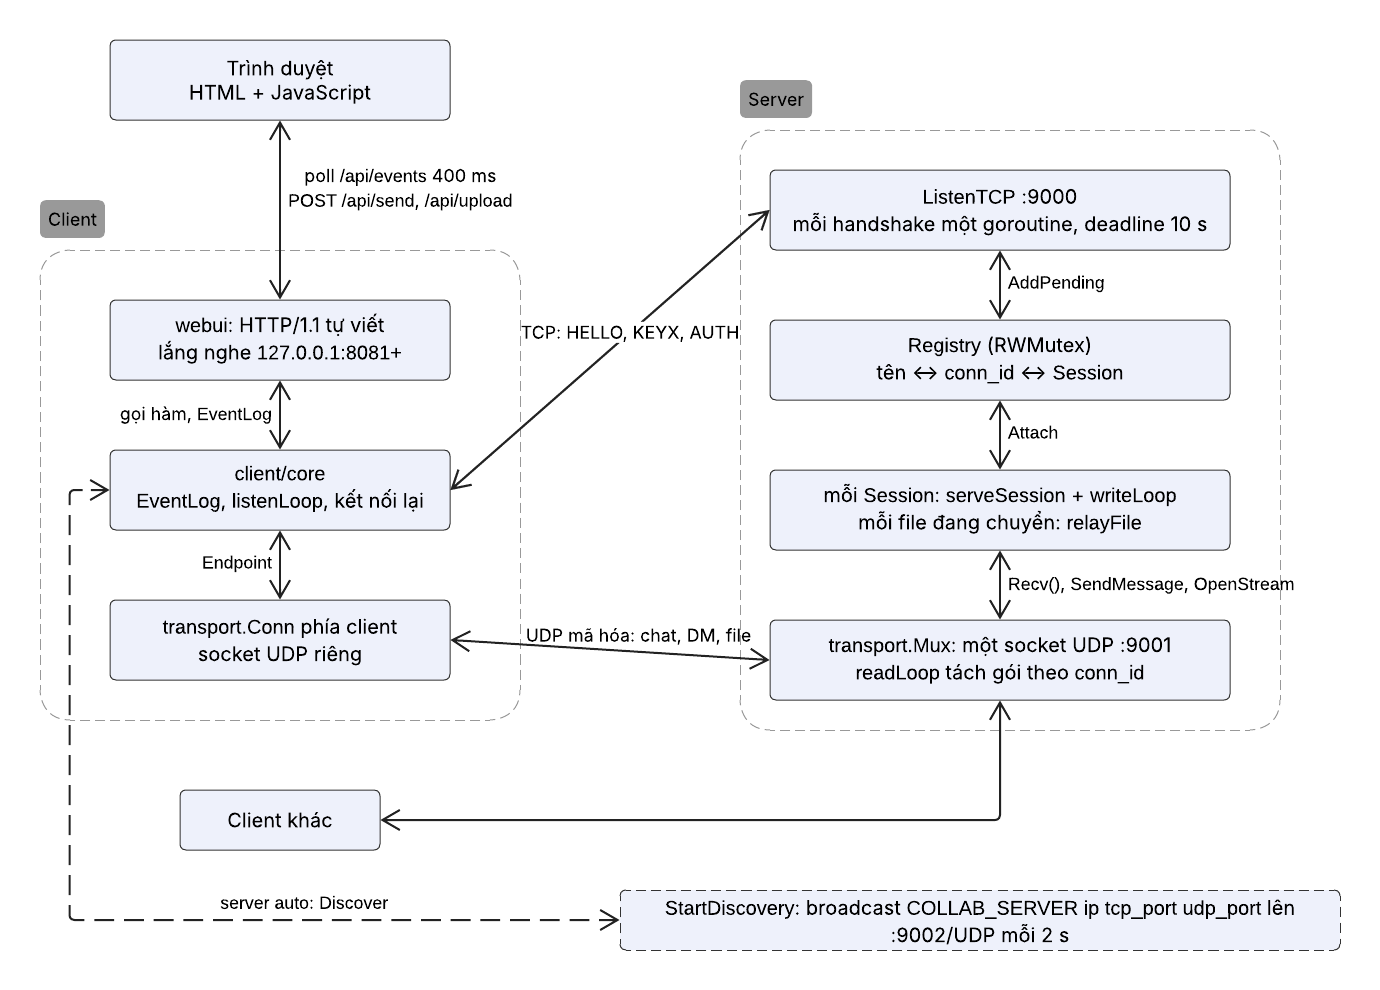
\includegraphics[width=\linewidth]{img/kien-truc.png}
  \caption{Kiến trúc chi tiết: các thành phần, goroutine chính và luồng dữ liệu}
  \label{fig:kien-truc}
\end{figure}

\paragraph{Phía Server.} Server chia thành ba nhóm goroutine chính:
\begin{enumerate}[label=(\arabic*), leftmargin=*, itemsep=2pt]
  \item \fname{ListenTCP} lắng nghe trên cổng 9000; mỗi lượt handshake chạy trong một goroutine riêng với deadline
        10 giây. Ngay sau khi xác thực thành công, server gọi \fname{Mux.Accept(conn\_id, $k_\text{udp}$)} để tạo
        đối tượng \fname{transport.Conn} cho kết nối UDP và gắn vào \fname{Session}.
  \item Mỗi session đang hoạt động có hai goroutine dài hạn: \fname{serveSession} đọc từ \texttt{Recv()} và phân
        loại stream theo byte đầu tiên (cắt tới cờ FIN rồi đưa đi định tuyến; luồng file được
        tách phần metadata ở đầu rồi chuyển tiếp từng mảnh sang goroutine \fname{relayFile} của file đó). Ở chiều
        ngược lại, \fname{writeLoop} là goroutine \emph{duy nhất} gọi \texttt{SendMessage} cho session này, lấy tin
        tuần tự từ hàng đợi \texttt{sendCh} (4096 phần tử) để giữ thứ tự gửi và cô lập các client nhận chậm
        (\cref{subsec:app}). Khi mới tạo phiên, một goroutine ngắn hạn \fname{watchPeer} chờ gói UDP đầu tiên của
        client để ghi nhận địa chỉ IP:port thực tế và phát lại danh sách user kèm địa chỉ mới cho cả phòng.
  \item \fname{Mux.readLoop} đọc gói từ socket UDP chung trên cổng 9001, tra trường \texttt{conn\_id} trong header
        để chuyển gói tới đúng đối tượng \fname{Conn}; mỗi \fname{Conn} có một goroutine \fname{run} riêng ở tầng
        transport.
\end{enumerate}
Danh sách người dùng online được lưu tại \fname{Registry} dưới khóa \texttt{RWMutex}. Các phương thức của
\fname{Registry} chỉ cập nhật hoặc chép nhanh danh sách (\fname{Snapshot}) rồi nhả khóa ngay trước khi gửi mạng,
tránh giữ khóa trong lúc I/O.

\paragraph{Phía Client.} Khi chạy với cờ \texttt{-server auto}, client lắng nghe gói UDP broadcast trên cổng 9002
(tối đa 5 giây) và lấy IP server từ địa chỉ nguồn của gói tin; socket bật \texttt{SO\_REUSEADDR}/\texttt{SO\_REUSEPORT}
để nhiều tiến trình client trên cùng máy có thể lắng nghe đồng thời. Khối \fname{client/core} giữ \fname{Endpoint}
hiện tại cùng goroutine \fname{listenLoop} ghép các stream nhận về, sắp lại thứ tự tin nhắn theo \texttt{Seq} và
ghi các sự kiện (chat, DM, danh sách user, tiến độ truyền file, trạng thái kết nối) vào \fname{EventLog} theo chỉ
số tăng dần. Nếu channel \texttt{Done()} đóng mà không do người dùng thoát, client chuyển sang trạng thái
\textsc{Reconnecting} và thực hiện handshake lại (\cref{subsec:state}).

\paragraph{Giao diện.} \fname{webui} là một HTTP/1.1 server nhóm tự viết trên \fname{net.Listen} (đọc request
line, header và body theo \texttt{Content-Length}), phục vụ trang HTML + JavaScript thuần nhúng sẵn vào file thực
thi. Trình duyệt poll \texttt{/api/events?since=N} để lấy sự kiện mới từ \fname{EventLog} (mỗi sự kiện có số thứ tự
tăng dần nên F5 hay mở nhiều tab không mất hoặc lặp tin) và \texttt{/api/status} để hiện RTT, cwnd, tỉ lệ mất gói.
File gửi đi được đẩy thẳng vào body của \texttt{POST /api/upload}. Luồng đi của một DM và một file qua các khối trên
được vẽ ở \cref{fig:seq-dm,fig:seq-file}; chi tiết cài đặt có trong \fname{docs/code-walkthrough.md}.
\IfFileExists{img/webui.png}{\Cref{fig:webui} là giao diện khi đang gửi file: cột trái là danh sách user
online kèm IP:port, giữa là tin nhắn theo tab (chat chung và từng DM) cùng thanh tiến trình file, thanh trên cùng
là trạng thái mạng (connected/reconnecting, RTT, cwnd, tỉ lệ mất gói).}{}

\IfFileExists{img/webui.png}{%
\begin{figure}[H]
  \centering
  \includegraphics[width=\linewidth]{img/webui.png}
  \caption{Giao diện web của client khi đang gửi file}
  \label{fig:webui}
\end{figure}}{}
